\documentclass[11pt]{article}
\usepackage{coling2020}
\usepackage{times}
\usepackage{url}
\usepackage{latexsym}
\usepackage[super]{nth}
\usepackage{color,soul}
\usepackage{multirow}
\usepackage{makecell}
\usepackage{textcomp}
\usepackage[toc,page]{appendix}
\usepackage{graphicx}

\colingfinalcopy

\title{Lexicographical Semantic Change Detection with BERT}

\author{Salih Furkan Akkurt \\
  Boğaziçi University \\
  Department of Computer Engineering \\
  34342 Bebek, Istanbul, Turkey \\
  {\tt furkan.akkurt@boun.edu.tr}
}

\date{}

\begin{document}
\maketitle
\begin{abstract}
  I publicly release the code and references in a repository~\cite{akkurt-2023-58t-app-repo}.
\end{abstract}

\section{Introduction}

Dictionaries are great sources of information related to languages.
They contain a lot of information regarding meanings (senses) of words.
As a language evolves, senses of its words change and dictionaries need to be updated accordingly.
Dictionary writers constantly work on manually detecting semantic changes in current usage.
This is a very time-consuming and expensive process.

In this work, I propose a method to automatically detect semantic changes in the English language by leveraging the contextualizing power of deep learning-based language models.
I use BERT~\cite{devlin-etal-2019-bert} to contextualize words in two corpora and cluster their contextualized representations to detect semantic changes.
The current proposed method in this paper does not detect if a sense of a word morphed into another sense but detects if a word has gained a new sense or lost one.
This method can be extended into detecting morphing of senses also.

\blfootnote{
    \hspace{-0.65cm}
    This work is licensed under a Creative Commons
    Attribution 4.0 International Licence.
    Licence details: \url{http://creativecommons.org/licenses/by/4.0/}.
}

\section{System Description}

\subsection{Data}

I use 3 types of data in my work.
The first type is a frequency list of words, the second a dictionary and the third corpora.

Firstly, I use the frequency list of words~\cite{word-freq-2023-coca} from the Corpus of Contemporary American English (COCA)~\cite{english-corpora-2008-coca}.
This list serves as my vocabulary which I use to detect semantic changes in.
I restrict my vocabulary to \textit{nouns} only.
There are 2635 nouns in the list, the most frequent three of which are \textit{man}, \textit{case} and \textit{money}.

Secondly, I use Merriam-Webster (MW)~\cite{mw-2023-dictionary} as my dictionary.
Merriam-Webster is a well-known dictionary that is updated quite frequently.
I have used its API~\cite{mw-2023-api} to get the sense counts of the words in my vocabulary.
These sense counts include all entries of the words, meaning with any parts of speech, not just nouns.
They serve two purposes: (1) to determine the semantic distance of the embeddings that is necessary for a sense distinction in dictionaries and (2) to, in the end, compare the number of senses of the words in the dictionary with the cluster counts of the word embeddings in the corpora.

Lastly, I use free samples~\cite{corpus-data-2023-corpora} of the COCA and the NOW corpus (News on the Web)~\cite{english-corpora-2016-now} as my two corpora that serve as the current usage of the language.
The COCA's sample has 8.9 million words of linear tokenized text and the one of the NOW's has 1.7 million words.
Content of the COCA ranges from academic usage to fiction and spoken language.
The NOW corpus is a collection of web-based news sources.
Since the task is detecting current semantic changes, the corpora should be recent.

\subsection{Method}

Firstly, the two corpora is merged into one.
When a given sentence is passed through BERT, each token of the sentence has its own contextual representation, as demonstrated by~\cite{pasini-etal-2020-clubert}.
I use BERT~\cite{devlin-etal-2019-bert} to contextualize words in the merged corpus and gather token representations of each word.
The implementation of BERT (base-uncased) on HuggingFace's Transformers~\cite{wolf-etal-2020-transformers} is used.
After this step, each word has its own sets of representations.
\cite{zhou-li-2020-temporalteller} used "the sum of the last 4 layers [of BERT] to encode both word meaning and context information".
Instead of summation, each representation is the concatenation of the last 4 layers of BERT's output in this work.
The representations are stored after a rounding operation to reduce the size of the data as the concatenation increases the size of the data by 4 times as opposed to summation.
Experiments showed that the rounding operation does not affect the results significantly.

After the contextualization step, the agglomerative clustering algorithm~\cite{Florek1951SurLL} is used to cluster the representations of each word.
The implementation of the algorithm on scikit-learn~\cite{scikit-learn} requires the number of clusters or the distance threshold to be specified.
I use the number of senses of the words in the dictionary as the number of clusters input to the algorithm.
The cosine distance metric is used to calculate the distances between these clusters.
The minimum distance between the clusters is then used as the distance threshold in the second clustering step.
This distance represents the semantic distance that compelled the dictionary writers to distinguish the senses of the word.

The second clustering step is the same with the first one except the distance threshold is used instead of the number of clusters.
This step is used to create new clusters without specifically knowing the number of clusters beforehand but the distance threshold.
In the agglomerative clustering algorithm, the distance threshold is the maximum distance between two clusters to be merged.
In the end, the number of clusters is the number of senses of the word represented in the corpora.

If the number of clusters of the second clustering is greater than the number of senses of the word in the dictionary, it means that the word has gained a new sense.
If the number of clusters is less than the number of senses of the word, it means that the word has lost a sense.
However, if the number of clusters is equal to the number of senses of the word, it does not mean that the word has not changed semantically, as it may have gained a sense and lost another at the same time.

\section{Experiments and Results}

\subsection{Cosine distance for semantic change detection}

First, I experimented on whether the cosine distance between the BERT representations of the words in the corpora can be used to detect semantic changes in the words.
I constructed two paragraphs with the word \textit{bank}, differing only in the middle sentences, one representing the financial sense of the word and the other the river bank sense.

\begin{itemize}
  \item First paragraph: I wake up early in the morning and start my day by having a cup of coffee and reading the news. After that, I take a shower and get dressed for work. I work from 9 to 5, and my job keeps me busy throughout the day. During my lunch break, I usually go for a walk in the park or grab a quick bite to eat at a nearby café. {\color{red} Today, I need to withdraw some cash, so I decide to go to the \textit{bank} during my lunch break. I walk to the \textit{bank}, which is just a few blocks away from my office, and withdraw the money that I need.} After that, I grab a sandwich and a soda and head back to the office to finish my work for the day. When I get home in the evening, I like to unwind by watching TV or reading a book. After dinner, I usually spend some time chatting with my family or friends before going to bed.
  \item Second paragraph (only the differing part): {\color{red} Today, since the weather is so hot, I decide to go to the river \textit{bank} to swim during my lunch break.}
\end{itemize}

The cosine distances between the representations of the word \textit{bank} in the two paragraphs are calculated.
Distances between usages:
\begin{itemize}
  \item Two usages in the first paragraph: 0.2214
  \item First usage in the first paragraph and the only usage in the second paragraph: 0.3990
  \item Second usage in the first paragraph and the only usage in the second paragraph: 0.4330
\end{itemize}

More experiments between several sentences with the same and different usages of words were conducted but the results are not consistent.
The cosine distances between the token representations are not reliable enough to detect semantic changes in the words.
Even though this is the case, I continued on to the next step of the method.

\subsection{Semantic change detection with BERT and clustering}

I have implemented the method described in the previous section completely and run it all the way through.
Minimum cosine distance between any 2 clusters for all the embeddings of the entire vocabulary turns out to be $0.0645$.
Using this minimum distance as the distance threshold, I have run the second clustering step.
This step yielded 11,081 clusters for the word \textit{time}.
The number of senses of the word \textit{time} in the dictionary is 23.
This means that the minimum distance that compelled the dictionary writers to create different senses in the dictionary is not representative of the entire semantic space.
If we use this small distance to cluster the embeddings, we end up with thousands of clusters for a single word, which is not useful for our purposes.

I have generated 2 T-SNE plots of the contextualized representations of the word \textit{time} after the first and second clustering steps, labels coming from the agglomerative clustering algorithm.
The first plot is shown in Figure~\ref{fig:time_1} and the second one in Figure~\ref{fig:time_2}.
One conjecture is that the cosine distances 

\begin{figure}
  \centering
  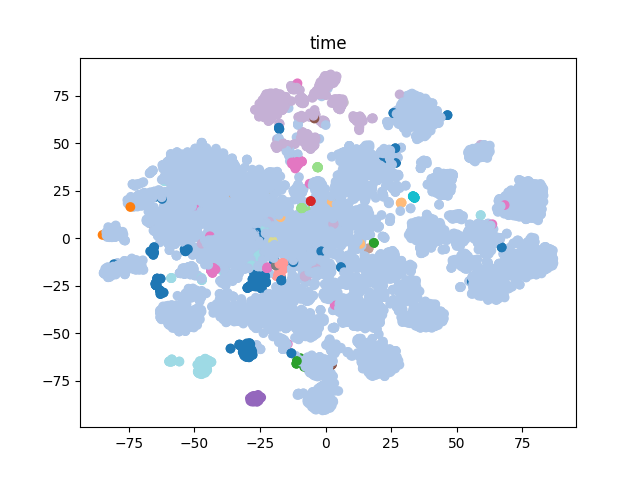
\includegraphics[width=0.8\textwidth]{time_1.png}
  \caption{The T-SNE plot of the contextualized representations of the word \textit{time} after the first clustering (number of clusters known) step.}
  \label{fig:time_1}
\end{figure}

\begin{figure}
  \centering
  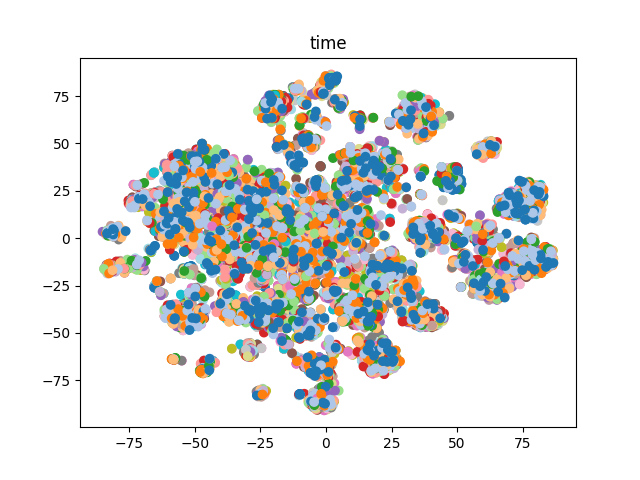
\includegraphics[width=0.8\textwidth]{time_2.png}
  \caption{The T-SNE plot of the contextualized representations of the word \textit{time} after the second clustering (distance threshold known) step.}
  \label{fig:time_2}
\end{figure}

\section{Discussion and Conclusion}

This work is a preliminary work on the topic of semantic change detection in lexicography.
The results are not very promising but the method is quite simple and can be improved upon.
The method can be improved by using a better clustering algorithm and a better distance metric.

For future work, with higher computational power, the whole COCA and NOW corpora instead of their samples can be used to represent a broader range of the current usage of the language.
Also, the vocabulary can be expanded to include other parts of speech such as verbs and adjectives.

To conclude, in this paper, I proposed a method to automatically detect semantic changes in words.
This method uses BERT to contextualize words in raw text and then clusters their contextualized representations to compare against the sense counts of the words in the dictionary.
As languages continuously change and dictionaries need updates quite frequently, this work can be used to help dictionary writers detect changes in language more efficiently.

\bibliographystyle{coling}
\bibliography{coling2020}

\end{document}
